\chapter{Track Classification MVA}\label{chap:track_classification_mva}

The chapter details work on implementing a multivariate algorithm (MVA) to predict the truth origin of reconstructed tracks.
An introduction to formalisms of machine learning is given in \cref{sec:ml_background}.
In \cref{sec:track_labelling}, the truth origin label is defined, and in \cref{sec:fake_track_mva} these labels are used to train a machine learning model that can effectively discriminate between good and fake tracks.
Several studies motivated this work by demonstrating that at high \pt, \btagging performance was degraded by the presence of large numbers of poorly reconstructed or fake tracks.
If an algorithm could be trained to detect fake tracks, these could be removed before their input to the \btagging algorithms with the aim of improving performance.


\section{Machine Learning Background}\label{sec:ml_background}

Over the past few decades, machine learning techniques have become increasingly popular in high energy physics experiments due the increased volumes of high-dimensional data and improvements in the field of machine learning (in particular deep learning).
Machine learning is the process in which a computer program automatically learns from data suitable parameters for a given model that can subsequently be used to to make predictions or inferences.
This is opposed to explicitly programming instructions on how to perform a specific task.
A subset of machine learning known as \textit{supervised learning} is used in this work, and consists of exposing a model to a number of labelled data samples and tasking the training algorithm with learning relationships between the input data and their labels.
These relationships are often complex, and explicitly programmed rules can fail to fully capture the relationships between inputs and outputs.

%The field of machine learning aims to design computer programs which, rather than being programmed explicitly with instructions on how to perform a specific task, instead learn from a set of labelled training examples $S_i$ how to perform the task for themselves, essentially replacing the need to manually design a program to perform a specific task.
%In this section a subset of machine learning techniques called supervised learning is described.

In the simplest case, a set of $m$ labelled training examples $S = \{ (x_1, y_1) , \ldots , (x_m, y_m) \}$ is collected.
Each element in the set $(x_i, y_i)$ consists of a input vector $x_i  \in \mathbb{R}^{\textnormal{input}}$, and the corresponding label $y_i$.
In classification problems, these labels are integer \textit{class labels} $y_i \in \{0,\ldots,N-1\}$, where $N$ is the number of classes, which specify which of a pre-determined set of categorical classes the training example belongs to.
The rest of the discussion in this chapter is limited to supervised classification problems where $N = 2$, i.e. binary classification.
Collecting sufficient and suitable data is one of the primary challenges of machine learning, as such data is not always readily available.
Fortunately, sophisticated tools to simulate particle collisions have already been developed by the scientific community \cite{leshouchesaccords, leshouchesstandardisation}. Simulation plays a key role in particle physics. More detail is given in.\todo{fix}


\subsection{Neural Networks}\label{sec:neural_nets}

After obtaining suitable training data, the next step is to define a model.
Given an input domain $\mathbb{R}^{\textnormal{input}}$ and an output domain $Y$, the model
$f: \mathbb{R}^{\textnormal{input}} \to Y$ is a parameterised functional mapping from input space to an output space.
In practice, $f$ is often implemented as a neural network, since these are easy to train via backpropagation.
Given an input example $x_i$ and a set of parameters $\bm{\theta}$, the model outputs a prediction $\hat{y}_i \in Y$ for the true label $y_i$, as in
%
\begin{equation}
    f(x_i, \bm{\theta}) = \hat{y}_i .
\end{equation}
%
In the case of binary classification ($N = 2$), the output domain $Y = (0, 1)$ is typically a single-dimensional scalar value.
The two classes are often referred to as signal ($y_i = 1$) and background ($y_i = 0$), which need to be separated.
The output $\hat{y}_i$ is in the interval $(0, 1)$ so as to be interpreted as the probability that the input example $x_i$ belongs to the signal class, rather than the background class.

The parameters $\bm{\theta}$ of the model are randomly initialised, however the model is designed to be expressive enough to correctly map the inputs $x_i$ to the outputs $y_i$ given the correct choice of parameters.
The model then undergoes a processes  called \textit{training}, which amounts to showing the model a series of labelled training examples and modifying the parameters of the model which belong to one of several categories.
The functional form of $h$ is chosen to maximise its effectiveness. Additionally specified are the coefficients of $h$, denoted $\bm\theta$, which are varied through the learning process to improve results. 

\subsubsection{Artificial Neurons}

The basic functional component of an ANN is the \textit{artificial neuron}, which is inspired by a mathematical model of a biological neuron \cite{mcculloch1943logical, hopfield1987neural}.
An artificial neuron is defined by its weights $\bm{\theta}$.
The neuron takes $n$ inputs and computes the dot product of the inputs and the weights and additionally adds a bias $\theta_0$.
The result is fed into an activation function.

\begin{figure}[!htbp]
    \centering
    \usetikzlibrary{matrix,chains,positioning,decorations.pathreplacing,arrows}
\begin{tikzpicture}[
    init/.style={
      draw,
      circle,
      inner sep=2pt,
      font=\Huge,
      join = by -latex
    },
    squa/.style={
      draw,
      inner sep=2pt,
      font=\Large,
      join = by -latex
    },
    start chain=2,node distance=13mm
    ]
    \node[on chain=2] 
      (x2) {$x_i^2$};
    \node[on chain=2,init] (sigma) 
      {$\displaystyle\Sigma$};
    \node[on chain=2,squa,label=above:{\parbox{2cm}{\centering Activation \\ function}}]   
      {$f$};
    \node[on chain=2,label=above:Output,join=by -latex] 
      {$\hat{y}$};
    \begin{scope}[start chain=1]
    \node[on chain=1] at (0,1.5cm) 
      (x1) {$x_i^1$};
    \end{scope}
    \begin{scope}[start chain=3]
    \node[on chain=3] at (0,-1.5cm) 
      (x3) {$x_i^3$};
    \end{scope}
    \node[label=above:\parbox{1.5cm}{\centering Bias \\ $\theta_0$}] at (sigma|-x1) (b) {};

    \draw[-latex] (x1) -- (sigma) node[midway,above] {$\theta_1$};
    \draw[-latex] (x2) -- (sigma) node[midway,above] {$\theta_2$};
    \draw[-latex] (x3) -- (sigma) node[midway,above] {$\theta_3$};
    \draw[o-latex] (b) -- (sigma);

    \draw[decorate,decoration={brace,mirror}] (x1.north west) -- node[left=10pt] {Inputs} (x3.south west);
\end{tikzpicture}
    \caption{
      A diagram displaying the logical flow of a single neuron with 3 inputs $x_i^j$.
      Each input is multiplied by a weight $\theta_i$, and the resulting values are summed.
      A bias term $\theta_0$ is added, and the result is passed to an activation function.
      Each neuron can be thought of as a logistic regression model.
    }
    \label{fig:neuron}
\end{figure}

The bias input $b$ is always equal to $b = 1$ and is modulated by the bias weight $\theta_0$. This term plays the role of a trainable constant value that is independent of the inputs.



The logistic regression model is a useful step to understanding an ANN. In essence, the logistic regression model amounts to a single neuron network. The gradient descent (\cref{sec:backprop_sgd}) algorithm is used to fit the model to the data. The predictor function $f$ has the linear form 
%
\begin{equation}\label{linear predictor}
    f(\mathrm{x}_i) = \theta_0 + \theta_1 \mathrm{x}_1 + \ldots + \theta_n \mathrm{x}_n 
    \bm{\theta} = \begin{pmatrix} \theta_0 , \theta_1 , \ldots , \theta_n \end{pmatrix}^T
    \mathbf{x} = \begin{pmatrix} 1 , \mathrm{x}_1 , \ldots , \mathrm{x}_n \end{pmatrix}^T .
\end{equation}
%
This expression can be written in terms of a vector dot product $f = \bm{\theta}^T \mathbf{x}$ if we express $\theta_j$ and $\mathrm{x}_i$ as vectors. The vector $\mathbf{x}$ has a $1$ as its $0^{\mathrm{th}}$ entry to give a constant term in the evaluation of $f$. This is known as the \textit{bias term}. As discussed, it only makes sense to obtain values in the interval $[0,1]$ from our model. As the predictor function is unbounded, it is intuitive to pass the output of the linear predictor to some bounded function. A common choice is the \textit{logistic function} $g(z)$, where
%
\begin{equation}\label{logistic}
    g(z) = \frac{1}{1 + e^{-z}} \implies g'(z) = g(z) [1 - g(z)] .
\end{equation}
%
The function $g(z)$ is known as the \textit{activation function}. A more detailed discussion on choice of activation function can be found in the next section. The application of $g(z)$ recovers the hypothesis function $h_\theta(\mathbf{x}) = g(\bm{\theta}^T \mathbf{x})$.



\subsubsection{Activation Functions}

As in their biological counterparts, the output of an artificial neuron cannot take any value - the neuron is either ``firing'' or ``not firing''. The role of the activation function is to compress neuron outputs between two boundaries. A naive way to do this is using the Heaviside step function (\ref{fig:activation_functions}), however this creates two problems. The first is that as the step function is linear, and as the hypothesis is built from several linear functions, we can only predict linear hypotheses. In this case the neural networks would fail to classify nonlinear data. The second problem is that the function has a vanishing (or infinite) gradient and is therefore not trainable. Instead, functions with a sigmoid shape are often employed. Some common examples are shown in \ref{fig:activation_functions}.

\begin{figure}[!htbp]
  \centering
  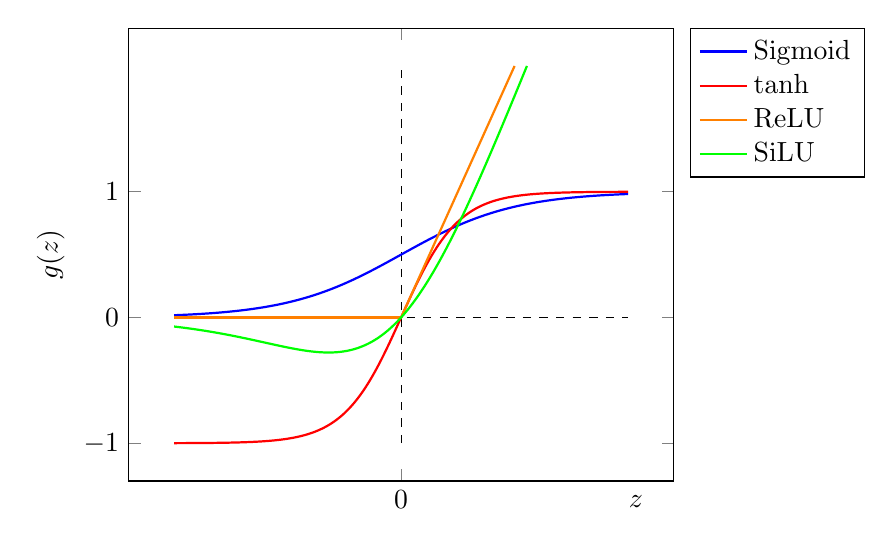
\begin{tikzpicture}
\pgfplotsset{width=8.5cm}
  \begin{axis}[
    domain=-4:4,
    xlabel=$z$,
    ylabel=$g(z)$,
    xtick={0},
    ytick={-1,0,1},
    every axis x label/.style={at={(0.9,-0.01)},anchor=north west},
    legend pos=outer north east,
    legend cell align=left
  ]
  % origin lines
  \addplot +[mark=none, black, dashed, forget plot] coordinates {(-4, 0) (4, 0)};
  \addplot +[mark=none, black, dashed, forget plot] coordinates {(0, -1) (0, 2)};

  % sigmoid 
  \addplot[thick, blue, samples=300] {1/(1+e^(-x))};%
  \addlegendentry{$\textnormal{Sigmoid}$}%

  % tanh
  \addplot[thick, red, samples=300] {tanh(x)};%
  \addlegendentry{$\textnormal{tanh}$}%
  
  % ELU
  %\addplot[thick, blue, samples=300, domain=-4:0, forget plot] {e^x - 1};%
  %\addplot[thick, blue, samples=300, domain=0:2] {x};%
  %\addlegendentry{$\textnormal{ELU}$}%

  % ReLU
  \addplot[thick, orange, samples=300, domain=-4:0, forget plot] {0};%
  \addplot[thick, orange, samples=300, domain=0:2] {x};%
  \addlegendentry{$\textnormal{ReLU}$}%

  % swish 
  % 1.278
  % 2.218
  \addplot[thick, green, samples=300, domain=-4:2.218] {x/(1+e^(-x))};%
  \addlegendentry{$\textnormal{SiLU}$}%

  \end{axis}%
\end{tikzpicture}
  \caption{A diagram displaying the logical flow of a single neuron with 3 inputs. Each neuron can be thought of as a logistic regression model.}
  \label{fig:activation_functions}
\end{figure}

The standard logistic function may not be as quick to train as choices that are asymmetrical about the origin, for example the hyperbolic tangent \cite{efficientbackprop}. The gradient of the activation function dictates how quickly the network can learn - the weight will not change much in areas where the gradient is small. The mean output of a layer with an antisymmetric activation function will be closer to $0$ than for a symmetric activation, and this is where sigmoidal functions have largest gradient. As such, the weight update is more likely to be larger for an antisymmetric function. This is also why data is normalised to have mean and standard deviation equal to 1 in the preprocessing stage.

Another activation function shown to have improvements over both the logistic function and $\tanh$ is the rectifier function. The Rectified Linear Unit (ReLU) were considered.



\subsubsection{Networks}

\subsubsection{Optimisation}


%
\begin{equation}\label{eq:bce_loss}
  J(\bm\theta) = -\frac{1}{m} \sum_{i=1}^m  \mathrm{y}_i \ln[h_\theta(\mathbf{x}_i)] + (1 - \mathrm{y}_i) \ln[1 - h_\theta(\mathbf{x}_i)] .
\end{equation}
%


\subsection{Backpropagation and Gradient Descent}\label{sec:backprop_sgd}

Finally a training algorithm must be developed to allow the program to improve its accuracy through exposure to the dataset. The function $h$ can then be used to predict categories for unseen data. Once the form of $h$ is fixed, the algorithm optimises the coefficients $\bm\theta$ to obtain the best results. The effectiveness of the trained classifier depends on the amount and quality of the training data in $S$, and the efficacy of the training algorithm. The training algorithm works by acting to minimise the \textit{cost function} $J(\bm\theta)$, which gives a measurement of the wrongness of $h$.


gradient descent is an example of an \textit{optimisation} algorithm that minimises the cost function $J(\bm\theta)$ (thereby fitting the logistic regression model discussed above to some data) by selecting the optimal values of $\bm\theta$. The algorithm works by computing the partial derivatives of $J(\bm{\theta})$ with respect to the parameters $\bm{\theta}$. The parameters are then altered slightly in the direction of decreasing slope, thereby reducing the cost function.
%
\begin{equation}\label{eq:weight_update}
    \theta_j \coloneqq \theta_j - \alpha \pd{}{\theta_j} J(\bm\theta)
\end{equation}
%
The parameter $\alpha$ is known as the \textit{learning rate} and dictates the size of the step taken in the direction of the slope. The above step must be performed simultaneously for each $\theta_j$ in $\bm{\theta}$, after which a new value of $J(\bm{\theta})$ can be calculated, and the process repeated. We can compute the partial derivatives of $J$ using the derivative of the logistic function from eq. \ref{eq:bce_loss}. The results are substituted into \cref{eq:weight_update} to obtain
%
\begin{equation}\label{cfpd}
    \pd{J(\bm\theta)}{\theta_j} = \frac{1}{m} \sum_{i=1}^m [h(\mathbf{x}_i) - \mathrm{y}_i] \mathrm{x}_j .
\end{equation}
%
There are many extensions and variations of the gradient descent algorithm. Some examples that provided better results in this project are described briefly below.
%
\begin{itemize}
    \item \textbf{Stochastic gradient descent} (SGD) performs a weight update after exposure to a fixed number of training examples, called a ``batch''. As such the cost function used is an approximation to eq. \cref{eq:bce_loss}. Standard gradient descent is unsuited to large datasets, and SGD has the advantage of introducing randomness from the approximation which means it can escape from local minima \cite{stochasticgrad}.
    %\item \textbf{Adaptive gradient descent} (AdaGrad) adds a learning rate for each weight in the network, so that neurons can learn at individual rates. Built into the algorithm is a reduction in step size over time, so learning slows as training progresses. This encourages good convergence \cite{adagrad}.
    \item \textbf{Adaptive Momentum} (Adam) accelerates SGD by dampening oscillations. A fraction of the previous weight update is used in the current update giving the process ``momentum'' \cite{2014arXiv1412.6980K}.
    %\item \textbf{RMSProp} is a variation of AdaGrad that removes the restriction that the learning rate must be reduced over time. Instead the learning rate depends only on a fixed number of the most recent gradients, and hence the value it can take is more flexible.
\end{itemize}





\section{Track Truth Origin Labelling}\label{sec:track_labelling}

Crucial to supervised learning techniques are are the ground truth class labels which the machine learning model is trained to predict.
, which are listed in \cref{tab:truth_origins}.

\begin{table}[!htbp]
    \footnotesize\centering
    \setlength{\tabcolsep}{0.5em} % for the horizontal padding
    \begin{tabular}{lll}
        \toprule 
        \textbf{Truth Origin} & \textbf{Description} \\
        \hline
        Pileup  & From a \pp collision other than the primary interaction \\
        Fake    & Created from the hits of multiple particles \\
        Primary & Does not originate from any secondary decay \\
        fromB   & From the decay of a \bhadron \\
        fromBC  & From a \chadron decay which itself is from the decay of a \bhadron \\
        fromC   & From the decay of a \chadron which is not from teh decay of a \bhadron \\
        %fromTau & From the decay of a $\tau$ \\
        OtherSecondary & From other secondary interactions and decays \\
        \bottomrule
    \end{tabular}
    \caption{
      Truth origins which are used to categorise the physics process that led to the production of a track.
      Tracks are matched to charged particles using the truth-matching probability~\cite{PERF-2015-08}.
      A truth-matching probability of less than $0.5$ indicates that reconstructed track parameters are likely to be mismeasured and may not correspond to the trajectory of a single charged particle.
      The ``OtherSecondary'' origin includes tracks from photon conversions, \Kshort and $\Lambda^0$ decays, and hadronic interactions.
    }
    \label{tab:truth_origins}
\end{table}

For the fake track classifier, the origins in \cref{tab:truth_origins} are used to construct a binary label by labelling all fake tracks which are not also fromB as background, and all other tracks (i.e. good tracks and fake fromB tracks) as signal.
The fake track classifier is then trained to distinguish between these two categories of tracks.
Fake tracks are defined using the \textit{truth-matching probability} (TMP), defined in \cref{eq:tmp_def}.
This is a weighted sum of the number of hits on a track which are from the same truth particle, versus the total number of hits on the track.
The weights are subdetector-dependent are designed to account for the varying number of layers in each of the subdetectors.
%
\begin{equation}\label{eq:tmp_def}
    \textnormal{TMP} = 
    \frac{
        10 N_{\textnormal{Pix}}^{\textnormal{good}} + 
        5  N_{\textnormal{SCT}}^{\textnormal{good}} + 
           N_{\textnormal{TRT}}^{\textnormal{good}}
        }{
        10 N_{\textnormal{Pix}}^{\textnormal{all}} + 
        5  N_{\textnormal{SCT}}^{\textnormal{all}} + 
            N_{\textnormal{TRT}}^{\textnormal{all}}
        }
\end{equation}
%


\section{Fake Track Identification Tool}\label{sec:fake_track_mva}


The rate of fake tracks increases at high transverse momentum as shown in \cref{fig:fakerate_vs_pt} due to the difficulties in track reconstruction outlined in \cref{sec:b_track_reco_challenges}.
Correspondingly, the performance of \btagging algorithms is reduced, as shown for SV1 in \cref{fig:sv1_perf_nofake}.

\begin{figure}[!htbp]
    \centering
    \includegraphics[width=0.5\textwidth]{chapters/track_classifier/figs/fakerate_vs_pt.pdf}
    \caption{
      Rate of fake tracks as a function of jet transverse momentum.
      The rate of fake tracks increases significantly as a function of \pt, and also increases as the distance to the jet axis decreases, and the number of tracks in the jet increases (not shown).
    }
    \label{fig:fakerate_vs_pt}
  \end{figure}
  
\begin{figure}[!htbp]
    \centering
    \includegraphics[width=0.7\textwidth]{chapters/track_classifier/figs/sv1_perf_nofake.pdf}
    \caption{
      The \ljet efficiency of the low level tagger SV1 as a function of \bjet efficiency for the nominal tracking setup (black) and for the case where fake tracks which are not from the decay of a \bhadron are removed.
      The \ljet efficiency is decreased, demonstrating that the presence of fake tracks is detrimental to algorithm performance.
    }
    \label{fig:sv1_perf_nofake}
  \end{figure}


\section{Conclusion}
todo: culmination of this work in the general classifier tool

Applications:
\begin{itemize}
    \item Frack to jet association
    \item Fake track studies (removal and for recommendations)
\end{itemize}

Improved with GNNs